% --- SECTION : CADRE MÉTHODOLOGIQUE ET PLANIFICATION DU PROJET ---
% Auteurs : ALGUI Rania — Projet : Automatisation de la Hotline (BOA)

\section{Cadre Méthodologique et Planification du Projet}
\label{sec:cadre_methodologique}

\subsection{Les rôles Scrum}
\label{subsec:roles_scrum}

Les rôles de la méthodologie Scrum sont :
\begin{itemize}
    \item \textbf{Scrum Master :} Le responsable du déroulement du processus. Il garantit l’efficacité de la collaboration entre les membres de l’équipe.
    \item \textbf{Product Owner :} Le représentant du client. Il détermine ce qui doit être réalisé.
    \item \textbf{Team :} Les développeurs chargés de la construction du logiciel et d’en faire une démonstration.
\end{itemize}

Dans le cadre de notre projet au sein de l'équipe IPA Factory, ces rôles ont été répartis comme suit :
\begin{itemize}
    \item \textbf{Product Owner :} Ce rôle est assuré par \textbf{M. Abdelouadoud CHAALI} (Chef de l’équipe IPA Factory et encadrant professionnel), qui détermine le périmètre fonctionnel du projet pour la Hotline BOA et valide sa conformité.
    \item \textbf{Scrum Master :} Ce rôle de facilitation est assuré par :
    \begin{itemize}
        \item \textbf{ALGUI Rania} (l'étudiante), pour le suivi méthodologique de ses propres sprints.
        \item \textbf{M. Hamza JANATE} (sous-encadrant), pour l'accompagnement quotidien, ses conseils et son aide à la résolution des obstacles techniques.
        \item \textbf{M. Mouhanad EL FILALI} (encadrant pédagogique), pour le suivi régulier et les conseils de structuration globale.
    \end{itemize}
    \item \textbf{Team :} Ce rôle est principalement porté par \textbf{ALGUI Rania} pour le développement du logiciel et les démonstrations de fin de sprint, en étroite collaboration sur les aspects techniques avec \textbf{Othmane KODDAM} et \textbf{Hajar ZARRIQ} (membres de l'équipe IPA Factory).
\end{itemize}

\subsection{Les réunions du processus Scrum}
\label{subsec:reunions_scrum}

La méthodologie SCRUM est composée de quatre réunions :

\begin{itemize}
    \item \textbf{Planification du Sprint :} La planification du sprint correspond à la réalisation d’un plan de sprint ou de release selon la capacité de la vélocité de l’équipe au listing des histoires utilisateurs prioritaires que l’équipe pense pouvoir réaliser au cours d’un sprint.
    \item \textbf{Revue de Sprint :} La revue du sprint a lieu en fin de sprint, l’équipe de développement présente les fonctionnalités terminées au cours du sprint et recueille les retours du représentant des utilisateurs finaux, c’est aussi à ce moment que la mise en place des prochains sprints peut être anticipée.
    \item \textbf{Rétrospective de Sprint :} La rétrospective de Sprint permet de faire un point sur le sprint en lui-même (productivité, efficacité, qualité...) afin de pouvoir s’améliorer pour les prochains sprints.
    \item \textbf{Mêlée quotidienne :} C’est une réunion quotidienne de 15 minutes qui permet au Scrum Master de faire le point sur le travail concernant les items du sprint en cours.
\end{itemize}

Afin de structurer le déroulement de ce projet, les tâches ont été planifiées sur une période allant de Février à Juin. Ce planning global est subdivisé en huit sprints de deux semaines chacun.

% Les figures ci-dessous (commentées car non disponibles) représentaient la chronologie des Sprints et le tableau Kanban sur Jira.
% \begin{figure}[htbp]
%     \centering
%     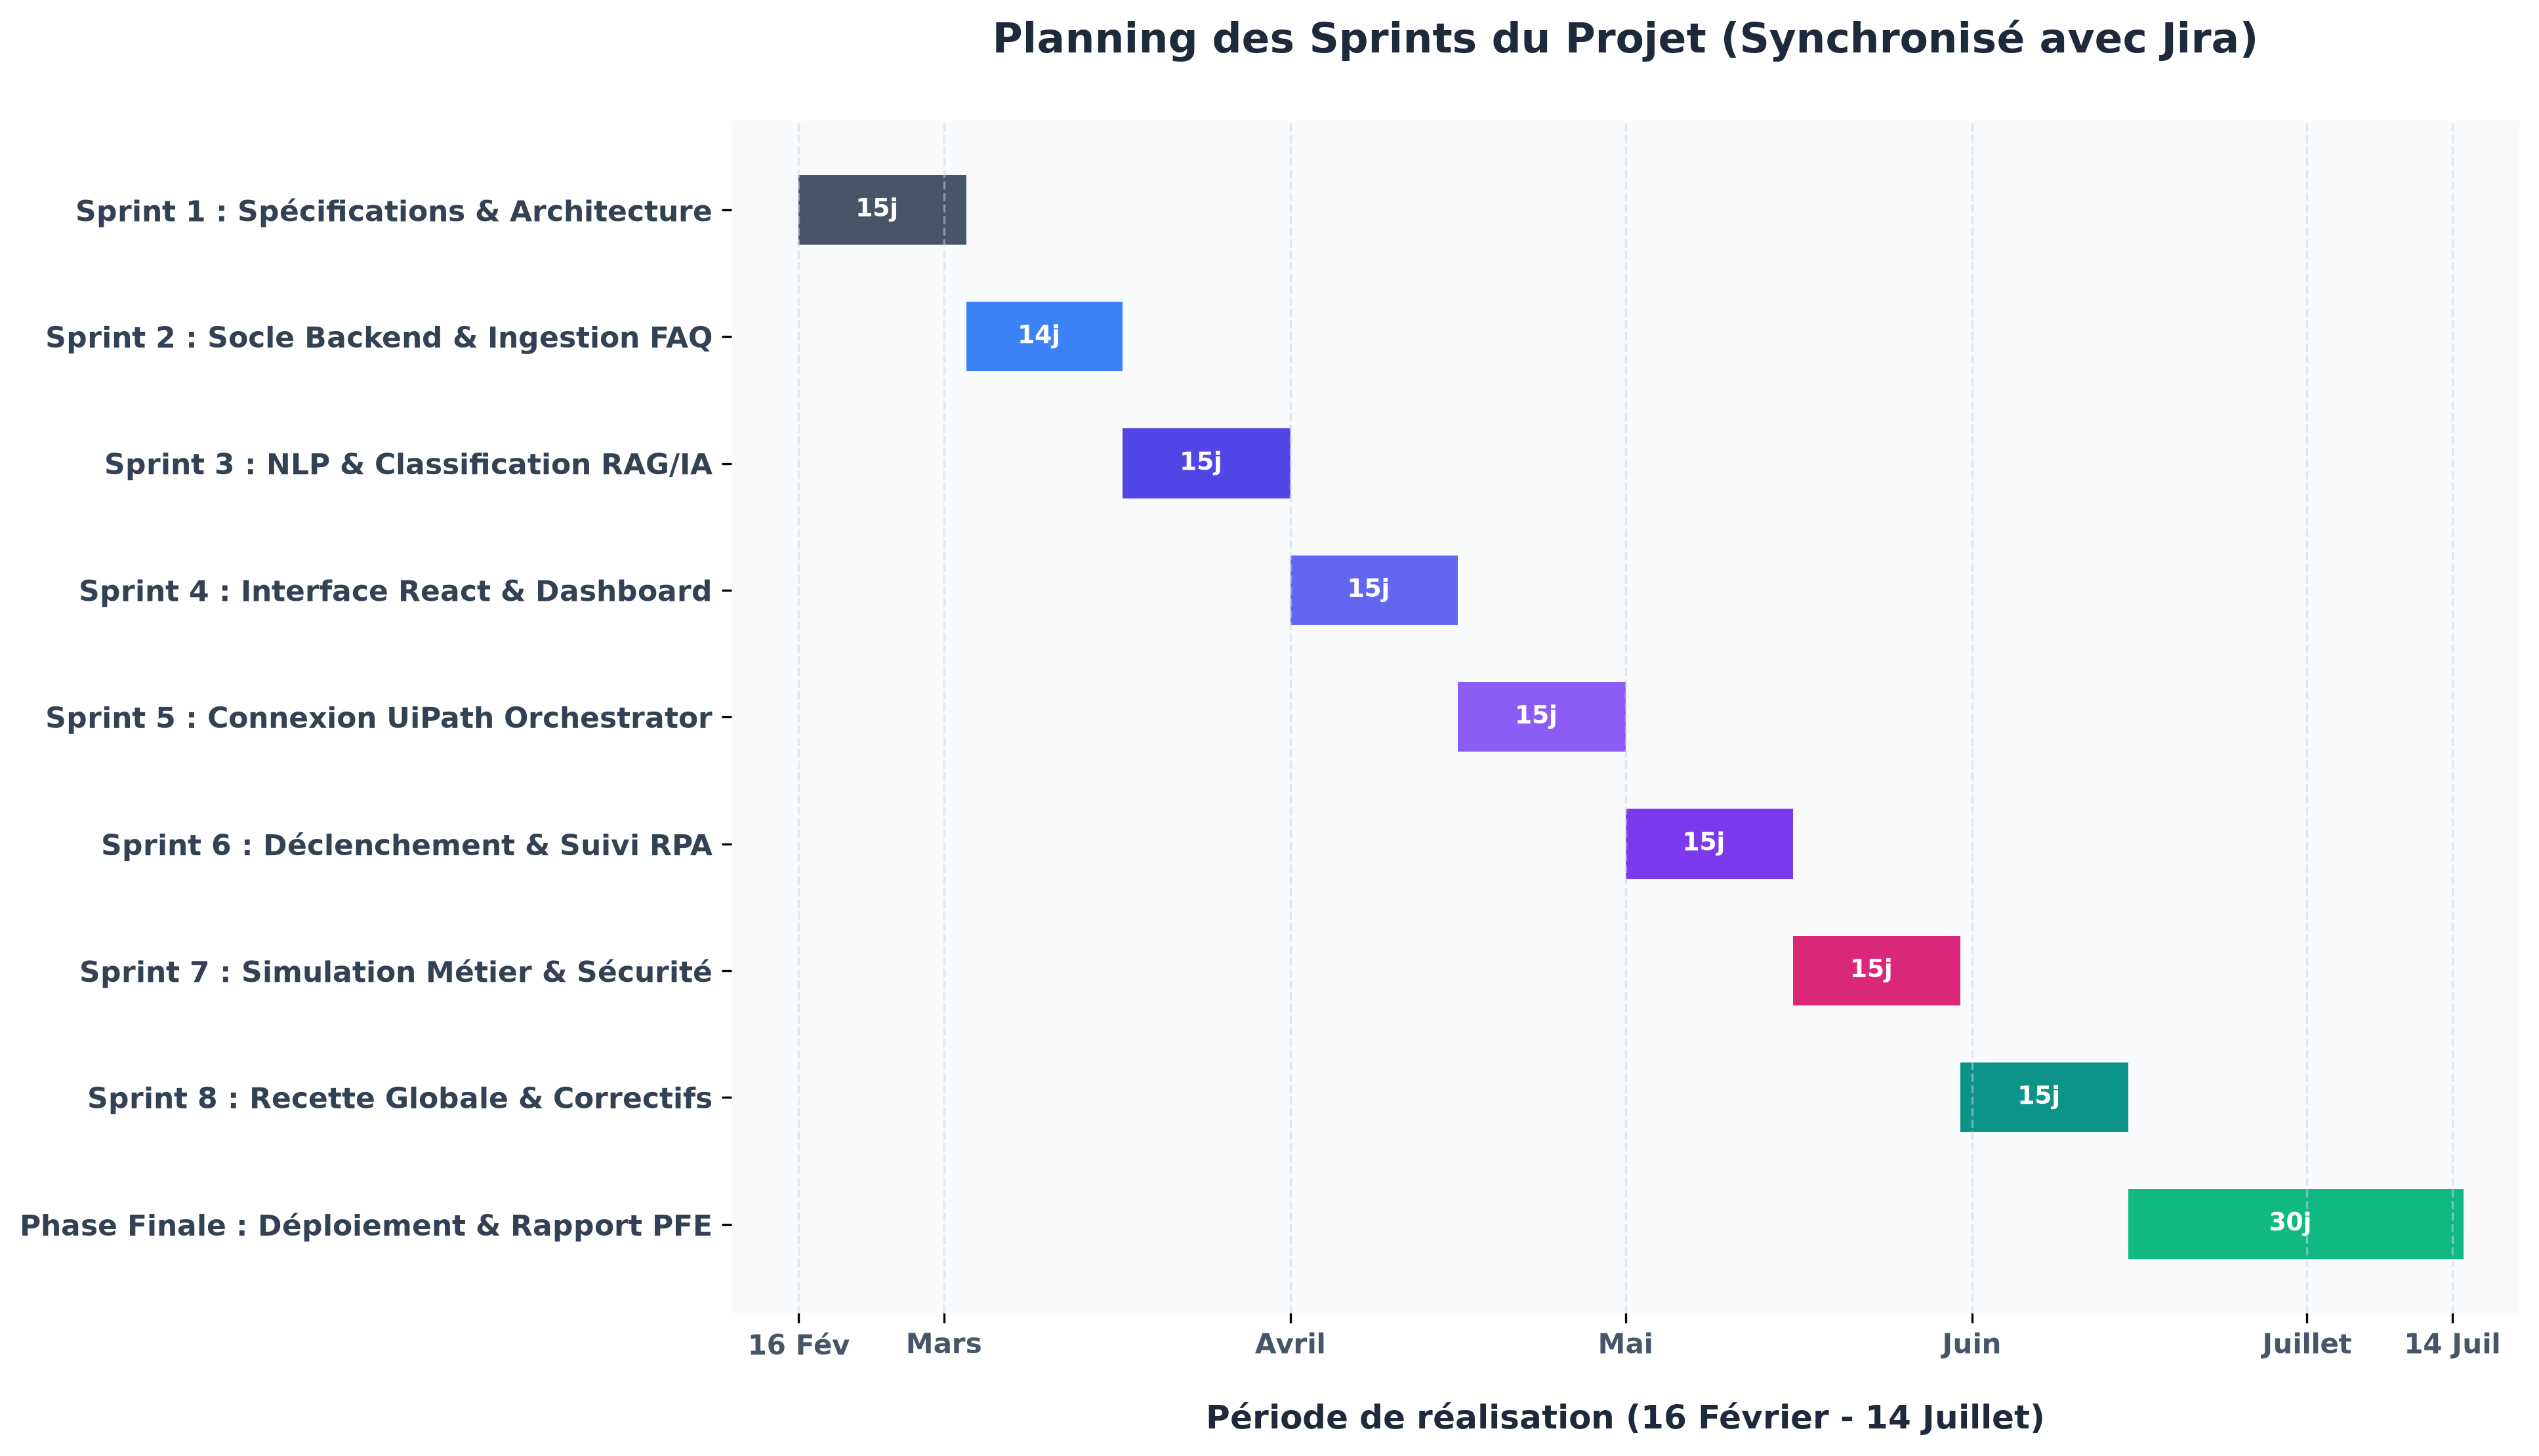
\includegraphics[width=\textwidth]{docs/sprints_timeline.png}
%     \caption{Planning des Sprints - ALGUI Rania (Février - Juin)}
%     \label{fig:sprints_timeline}
% \end{figure}
%
% \begin{figure}[htbp]
%     \centering
%     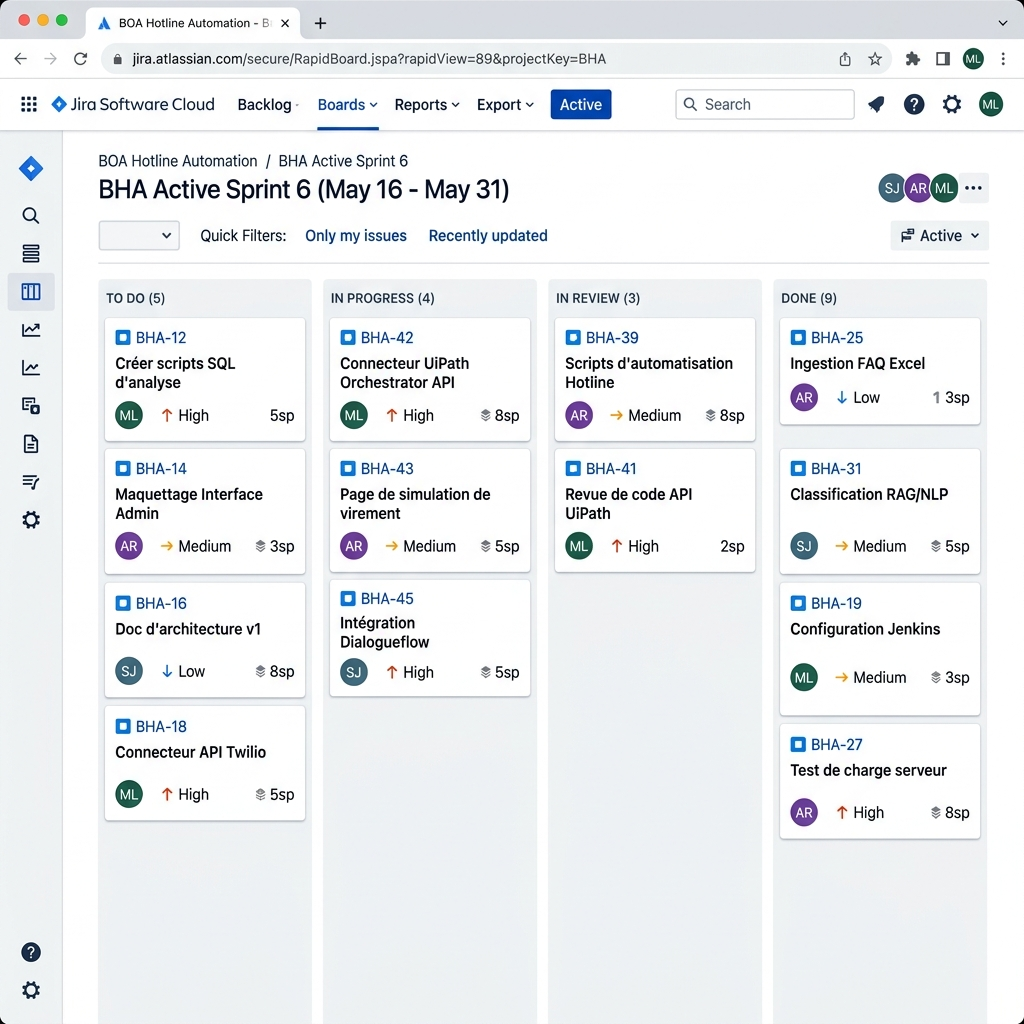
\includegraphics[width=0.95\textwidth]{docs/jira_scrum_board.png}
%     \caption{Suivi du Sprint Backlog du Projet sur Jira}
%     \label{fig:jira_scrum_board}
% \end{figure}

\subsubsection{Déroulement pratique des rites Scrum : Exemple du Sprint 3}
\label{subsubsec:exemple_pratique_scrum}

Bien que ce projet de fin d'études ait été réalisé de façon individuelle, les rites Scrum ont été simulés et appliqués rigoureusement afin de structurer le déroulement des tâches et d'assurer une communication fluide avec l'encadrement. 

Pour illustrer cette démarche, nous présentons ci-dessous le déroulement des quatre cérémonies Scrum lors du \textbf{Sprint 3} (du 16 au 29 Mars), qui a porté sur le développement du module d'intelligence artificielle (RAG/NLP) et la classification des requêtes.

\begin{enumerate}
    \item \textbf{Planification du Sprint 3 (Sprint Planning) :}
    \begin{itemize}
        \item \textbf{Date \& Durée :} 16 Mars 2026 (2 heures)
        \item \textbf{Participants :} ALGUI Rania (Développeuse / Scrum Master), Encadrant professionnel BOA (Product Owner).
        \item \textbf{Objectif du Sprint :} Mettre en place la classification automatique des requêtes par IA et l'API de recherche FAQ.
        \item \textbf{Contenu de la réunion :} Analyse du Product Backlog et estimation de l'effort de développement. Les User Stories suivantes ont été sélectionnées :
        \begin{itemize}
            \item \textbf{US-06} (Classification N1-RR par IA) : Estimée à 8 Story Points (effort important lié à l'intégration du NLP/RAG).
            \item \textbf{US-07} (Recherche FAQ en langage naturel) : Estimée à 5 Story Points (s'appuyant sur les données déjà structurées).
        \end{itemize}
        L'équipe s'est engagée sur une vélocité totale de \textbf{13 Story Points}. Les tâches techniques ont été découpées et assignées sur Jira.
    \end{itemize}

    \item \textbf{Mêlée quotidienne (Daily Scrum) :}
    \begin{itemize}
        \item \textbf{Date \& Durée :} 23 Mars 2026 (15 minutes)
        \item \textbf{Participants :} ALGUI Rania (Développeuse).
        \item \textbf{Contenu de la réunion (Auto-suivi) :}
        \begin{itemize}
            \item \textit{Travail réalisé la veille :} Finalisation du script Python de recherche sémantique sur la base FAQ Excel.
            \item \textit{Travail prévu pour la journée :} Création de l'API REST dans le backend Spring Boot pour l'intégrer au chatbot.
            \item \textit{Obstacles rencontrés :} Lenteurs de chargement du modèle sémantique lors des premières requêtes. Solution retenue : optimiser la mise en cache des embeddings.
        \end{itemize}
    \end{itemize}

    \item \textbf{Revue de Sprint 3 (Sprint Review) :}
    \begin{itemize}
        \item \textbf{Date \& Durée :} 28 Mars 2026 (1 heure)
        \item \textbf{Participants :} ALGUI Rania (Développeuse), Encadrant BOA (Product Owner), Conseillers Hotline BOA (Utilisateurs pilotes).
        \item \textbf{Contenu de la réunion :} Démonstration des fonctionnalités terminées du chatbot. Saisie en direct de la question : \textit{« Comment réinitialiser le mot de passe BOA-Net ? »}. Le chatbot a correctement identifié la panne comme N1-RR et retourné la solution FAQ en moins d'une seconde.
        \item \textbf{Décision :} Le Product Owner a validé les critères d'acceptation et a marqué les US-06 et US-07 comme « Terminées » (Done).
    \end{itemize}

    \item \textbf{Rétrospective de Sprint 3 (Sprint Retrospective) :}
    \begin{itemize}
        \item \textbf{Date \& Durée :} 29 Mars 2026 (45 minutes)
        \item \textbf{Participants :} ALGUI Rania (Développeuse).
        \item \textbf{Contenu de la réunion (Bilan méthodologique) :}
        \begin{itemize}
            \item \textit{Points positifs :} Le travail de préparation des données FAQ au Sprint 1 a permis de coder l'API d'IA très rapidement.
            \item \textit{Points à améliorer :} Perte de temps sur les configurations proxy pour contacter l'Orchestrator UiPath (anticipation du Sprint 5).
            \item \textit{Action corrective pour le Sprint 4 :} Ouvrir les accès et tester la connectivité réseau avec le service informatique dès le début du prochain sprint.
        \end{itemize}
    \end{itemize}
\end{enumerate}


\subsection{Product backlog}
\label{subsec:product_backlog}

Le Product backlog correspond à une liste priorisée des besoins et des exigences du client. Les éléments du backlog de produit, appelés aussi les histoires utilisateurs (\textit{User Stories}), sont formulés en une ou deux phrases décrivant de manière claire et précise la fonctionnalité désirée par le client, généralement écrit sous la forme : 
\begin{center}
    \textit{« En tant que [Acteur], je veux [Fonctionnalité], afin de [Bénéfice] »}
\end{center}

Dans le cadre de la mise en œuvre itérative et agile de ce projet de fin d’études, le tableau~\ref{tab:product_backlog} présente le backlog produit pour organiser et prioriser les différentes fonctionnalités à développer. Ce backlog prend la forme d’User Stories, qui décrivent les attentes des divers acteurs du système (développeuse, robot, responsable support, etc.) ainsi que les fonctionnalités qui y sont liées. Chaque User Story est également dotée d’une priorité (Must / Should), d’un sprint de réalisation, et d’un critère d’acceptation pour assurer une validation efficace.

Ce découpage nous aide à structurer les deux grandes missions du projet :
\begin{enumerate}
    \item \textbf{La supervision intelligente des applications via RPA} (intégration avec UiPath).
    \item \textbf{L’analyse des tickets IT enrichie par l’IA} (chatbot + RAG/NLP).
\end{enumerate}

\begin{table}[htbp]
\centering
\small
\begin{tabular}{|l|p{2cm}|p{2cm}|p{4.5cm}|c|c|p{3.5cm}|}
\hline
\textbf{ID} & \textbf{Mission} & \textbf{Rôle} & \textbf{Description (User Story)} & \textbf{Prio.} & \textbf{Sprint} & \textbf{Critère d'acceptation} \\ \hline
US-01 & Cadrage & Développeuse & En tant que dév, je veux analyser les cas d'usage afin de définir le périmètre automatisable. & Must & Sprint 1 & Liste des cas N1-RR et N2 validée. \\ \hline
US-02 & Cadrage & Développeuse & En tant que dév, je veux me former sur UiPath afin de maîtriser les outils RPA. & Must & Sprint 1 & Cours UiPath Academy validés. \\ \hline
US-03 & Cadrage & Développeuse & En tant que dév, je veux nettoyer les données afin de construire une base FAQ propre. & Should & Sprint 1 & Fichier Excel FAQ structuré sans doublons. \\ \hline
US-04 & Cadrage & Développeuse & En tant que dév, je veux concevoir l'architecture Spring Boot/React afin de poser les bases de l'app. & Must & Sprint 2 & Projets initialisés sur Git. \\ \hline
US-05 & Cadrage & Resp. Support & En tant que resp, je veux définir les flux N1-RR afin de préparer les spécifications du robot. & Must & Sprint 2 & Schémas de flux d'incidents validés. \\ \hline
US-06 & Analyse IA & Conseiller & En tant que conseiller, je veux que le chatbot classifie ma requête afin d'obtenir le bon canal. & Must & Sprint 3 & Module RAG/NLP classant les cas N1-RR avec précision $>$ 85\%. \\ \hline
US-07 & Analyse IA & Conseiller & En tant que conseiller, je veux interroger la FAQ en langage naturel afin d'obtenir des réponses rapides. & Must & Sprint 3 & API FAQ active avec temps de réponse $<$ 1s. \\ \hline
US-08 & Analyse IA & Resp. Support & En tant que resp, je veux un moteur de décision automatique afin d'orienter l'utilisateur sans intervention. & Must & Sprint 4 & Moteur fonctionnel selon le type de panne. \\ \hline
US-09 & Analyse IA & Développeuse & En tant que dév, je veux écrire des tests unitaires afin de garantir la qualité et stabilité du code. & Should & Sprint 4 & Couverture de test du moteur de décision $>$ 70\%. \\ \hline
US-10 & Supervision RPA & Développeuse & En tant que dév, je veux l'authentification OAuth2 afin de sécuriser les requêtes vers l'Orchestrator. & Must & Sprint 5 & Jeton d'accès de l'Orchestrator récupéré automatiquement. \\ \hline
US-11 & Supervision RPA & Resp. Support & En tant que resp, je veux déclencher le robot UiPath via l'API afin de résoudre la panne N1-RR immédiatement. & Must & Sprint 6 & Requête POST StartJob retournant un job\_key unique. \\ \hline
US-12 & Supervision RPA & Développeuse & En tant que dév, je veux journaliser les statuts des robots afin de suivre et déboguer les exécutions. & Should & Sprint 6 & Polling de statut fonctionnel avec logs en base. \\ \hline
US-13 & Sécurité & Resp. Sécurité & En tant que resp. sécu, je veux masquer les données bancaires afin de garantir la conformité. & Must & Sprint 7 & Masquage automatique des cartes dans l'UI et les logs. \\ \hline
US-14 & Simulation & Développeuse & En tant que dév, je veux un simulateur de virement/blocage afin de valider l'envoi de données au robot. & Should & Sprint 7 & Formulaires de simulation fonctionnels en React. \\ \hline
US-15 & Recette & Conseiller & En tant que conseiller, je veux tester l'application afin de valider son bon fonctionnement avant le pilote. & Must & Sprint 8 & Recette utilisateur (UAT) validée sans bug bloquant. \\ \hline
US-16 & Clôture & Développeuse & En tant que dév, je veux rédiger la documentation technique afin de faciliter la maintenance du projet. & Must & Sprint 8 & Manuel d'installation et d'administration livré. \\ \hline
\end{tabular}
\caption{Product Backlog Détaillé du Projet (Format User Stories)}
\label{tab:product_backlog}
\end{table}

\subsection{Planification des sprints}
\label{subsec:planification_sprints}

Afin de mener à bien ce projet dans le respect des délais et des contraintes de qualité, nous avons adopté la méthodologie Agile Scrum. Le projet est découpé en \textbf{huit sprints} distincts d’une durée de \textbf{deux semaines chacun}, s’étalant sur une période globale de \textbf{seize semaines (quatre mois)} du \textbf{16 Février au 14 Juillet} (la période restante étant allouée à la phase finale de déploiement, recette utilisateur et rédaction du rapport de PFE).

Le tableau~\ref{tab:sprint_planning} détaille cette planification ainsi que les objectifs, les activités clés et les livrables associés à chaque sprint. Cette approche itérative nous permet de suivre de manière rigoureuse la transition entre les phases d’analyse et de conception, de développement du cœur backend et de l’intelligence artificielle, d’intégration avec l’environnement RPA d’UiPath, et enfin de validation utilisateur avant la livraison de la solution finale.

\begin{table}[htbp]
\centering
\small
\begin{tabular}{|l|l|p{3cm}|p{4.5cm}|p{3.5cm}|}
\hline
\textbf{Sprint} & \textbf{Période} & \textbf{Objectifs} & \textbf{Activités Clés} & \textbf{Livrables} \\ \hline
Sprint 1 & 16 Fév – 01 Mar & Cadrage \& Formation & Analyse des besoins hotline BOA ; formation UiPath Academy ; nettoyage des données. & Liste des cas d'usage validée ; environnement prêt. \\ \hline
Sprint 2 & 02 Mar – 15 Mar & Conception \& Architecture & Conception de l'architecture technique ; initialisation Spring Boot/React ; définition des flux. & Projets initialisés sur Git ; diagrammes de flux validés. \\ \hline
Sprint 3 & 16 Mar – 29 Mar & Classification IA \& FAQ & Développement du traitement RAG/NLP ; classification des requêtes N1-RR ; API REST FAQ. & Module de classification IA prêt ; API FAQ opérationnelle. \\ \hline
Sprint 4 & 30 Mar – 12 Avr & Moteur de décision \& Tests & Implémentation du moteur de décision backend ; écriture des tests unitaires sur le backend. & Moteur de décision fonctionnel ; couverture de test $>$ 70\%. \\ \hline
Sprint 5 & 13 Avr – 26 Avr & Connexion Orchestrator & Authentification OAuth2 (Client Credentials) ; client HTTP de connexion UiPath. & Module d'authentification Orchestrator validé. \\ \hline
Sprint 6 & 27 Avr – 10 Mai & Déclenchement RPA \& Suivi & APIs de démarrage de Job et de suivi du statut des robots ; logs d'intégration. & Endpoints de déclenchement et de polling RPA opérationnels. \\ \hline
Sprint 7 & 11 Mai – 24 Mai & Simulation \& Sécurité & Pages React de simulation bancaire ; masquage des données sensibles ; logs d'audit. & Simulation active ; logs et masquage configurés. \\ \hline
Sprint 8 & 25 Mai – 07 Juin & Recette technique \& Docs & Tests d'intégration end-to-end ; recette utilisateur ; rédaction de la documentation technique. & Prototype end-to-end validé ; manuel technique livré. \\ \hline
Clôture & 08 Juin – 14 Juil & Déploiement \& Rapport & Installation pilote ; tests hotline ; rédaction du rapport final de PFE. & Rapport PFE validé et livrable prêt pour pilote. \\ \hline
\end{tabular}
\caption{Planification Détaillée des Sprints (Tableau 2.2)}
\label{tab:sprint_planning}
\end{table}
 obituary.tex
